\documentclass[12pt, letterpaper]{article}
\usepackage[utf8]{inputenc}
\usepackage{graphicx}
\usepackage[T1]{fontenc}
\usepackage{listings} \lstset{language=c, showstringspaces=false, xleftmargin=-60pt, frame=l}
\usepackage{url}

\graphicspath{ {/} }



\title{Green Threads ID1206 Operating Systems}
\author{Frida Johansson}
\date{December 2021}

\begin{document}

\maketitle
\section{Introduction}
This task was about to implement our own thread library. Instead of using the OS POSIX threads we
created our own scheduler and context handler. The task was divided into several parts where
new implementations was implemented each time which will be briefly explained in each section.
When the last implementation was implemented a benchmark was done to measure the time it took to 
execute the program using our own green thread implementation compared to the pthread library. 

\section{Implementations}
To be able to use a context it must be initiated first. That is handled by the function 
\emph{makecontext()} where the main context will be initiated while the program is loaded. 

A first implementation of the program was to call function \emph{yield()} which suspended
a running thread, put it on the Ready Queue and switched context. The Ready queue in this implementation 
was made of two pointers, one pointing at the first thread on the queue and the other pointing at the last thread.
This was implemented this way to handled the \emph{enqueue()} and \emph{dequeue()} functions in O(1) time. 
The Ready queue will in the tests not be long since only two threads will be running but
if several threads would be implemented, this would be better for the time performance. Otherwise, if the Ready Queue only had one pointer pointing at the head 
the time complexity for \emph{enqueue()} and \emph{dequeue()} would be proportional to the length of the Ready Queue.

\subsection{Suspending on a condition}

The implementation of conditional variables is implemented as a data structure with two pointers.
One pointing to the first thread on the suspended queue and one pointing on the last thread. This
data structure is used when a state is not desired and the current running thread can suspend on the condition. 
If a shared buffer would be used between two threads, one consumer and one producer, a challenge 
is to prevent the producer from trying to write to the buffer when full, and prevent the consumer to 
read the buffer when empty. This will be handled later when we notice some weird behaviour when interrupts are implemented.

\subsection{Timer interrupts}
To make life hard, but efficient if it works, a timer interrupt was implemented to enable concurrent execution
among several threads. This interrupt was set to a period of 100 and every period a timer handler was called
that worked exactly as the \emph{yield()} function. To prevent a timer interrupt while handling state of our green threads
we blocked and unblocked the interrupts with the help of \emph{sigprocmask()} funktion.
However this does not solve the problem when data is shared among threads. This only made it harder since
we could now get a timer interrupt while updating our data structures which could end up really badly. 

\subsection{Mutex}
To solve this matter of shared data structures a mutex was implemented. The mutex data structure consisted of
a volatile int that worked as a lock and two pointers representing the suspended list of threads. One pointer
pointing at the first thread of the list and one pointer poining at the last thread of the list. 

\section{Performance}

\subsection{Before atomic operation}
With all implementations done a test program was written to ensure that everything worked well.
Unfortunately it behaved very strange. Why? A timer interrupt was executed just after we unlocked the mutex with \emph{green{\_}mutex{\_}unlock()}
and before we got in to \emph{green{\_}cond{\_}wait()}. To prevent this behaviour we want these two functions to execute as an 
atomic operation like the pthreads library funtion \emph{pthread{\_}cond{\_}wait()} where both the conditional variable
and the mutex is sent as arguments. 

\subsection{After Adjustments - No more seg faults}
Following two figures of c code shows the implementation of the producer and consumer where the funtion \emph{green{\_}cond{\_}wait()} now takes two argument
instead of one and is now an atomic operation to prevent a timer interrupt. The bench program initializes both our green threads and
pthreads to compare the execution time between them two. A producer and consumer function was written for the pthreads as well that made use of the pthreads library. 
I had a huge problem with this implementation. In the wait function when we was suppose to handle mutex I called the 
function \emph{green{\_}mutex{\_}unlock()} which handled the data structures as desired but one detail I did not think of that made a huge difference was that
the function also unblocked the block which was the opposite what we wanted since interrupts now could interfere. It might sound obvious for the reader but while implementing 
this I did not see this detail. To solve this I implemented the code from \emph{green{\_}mutex{\_}unlock()} in \emph{green{\_}cond{\_}wait()} and in that way keeping interrupts blocked. 


\begin{lstlisting}[
    basicstyle=\small]

void* producer(void* arg){
    int id =*(int*)arg;
    int i;
    for (i = 0; i < productions; i++){
        green_mutex_lock(&mutex);
        while (count == 1){
            green_cond_wait(&empty, &mutex);
        }
        count = 1;
        green_cond_signal(&filled); 
        green_mutex_unlock(&mutex);
    }
return (void*) 0; 
}

void* consumer(void* arg){
    int id =*(int*)arg;
    int i;
    for (i = 0; i < productions; i++){
        green_mutex_lock(&mutex);
        while (count == 0){
            green_cond_wait(&filled, &mutex);
        }
        count = 0;
        green_cond_signal(&empty); 
        green_mutex_unlock(&mutex);
    }
    return (void*) 0; 
}
    \end{lstlisting}

    To bench the exection time between pthreads and green threads a clock was set each execution and a production counter increased by 100
    productions each execution in the beginning and by 500 productions when the counter had reached 500. In the next two graphs on the following page you will see 
    the result from the bench program where one uses one core and the other uses multiple cores. 

\begin{figure}[h]
    \center
    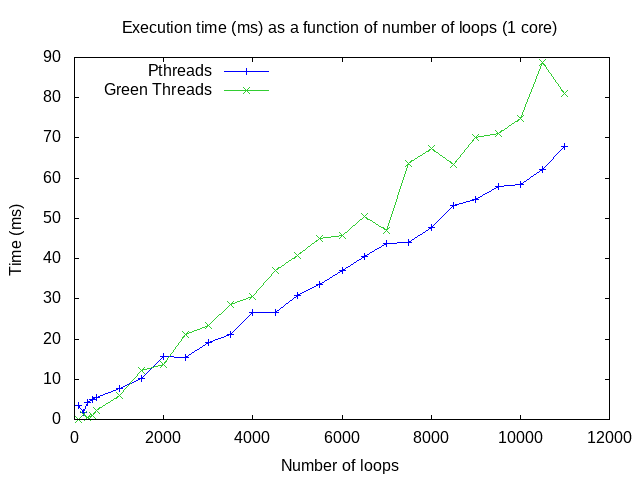
\includegraphics[scale=0.6]{unicore.png}
    \caption{Performance One Core}
    \label{fig:graph1}
\end{figure}

\begin{figure}[h]
    \center
    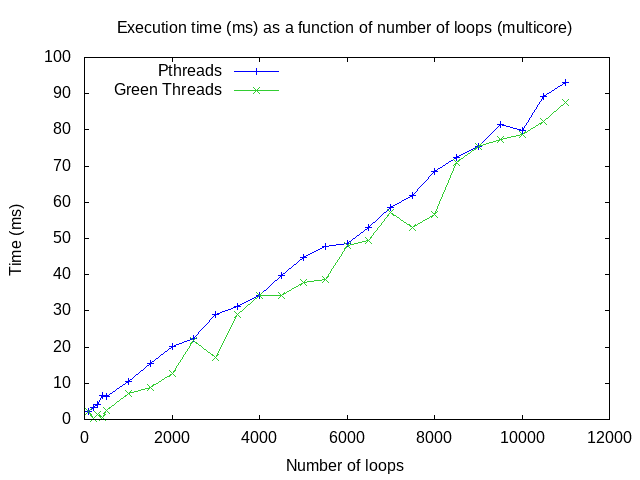
\includegraphics[scale=0.6]{multicore.png}
    \caption{Performance multiple cores }
    \label{fig:graph0}
\end{figure}



\section{Result and Discusson}
Green threads only exists in the user space which is (almost) what we implemented if we don't mention \emph{swapcontext()} which
make use of OS threads. Pthreads stands for POSIX threads and is the default standard in the UNIX systems. 
When looking at the performance graph for the multicore bench program the green threads performed slightly better
than pthreads. An answer for that could be that we are only in the user space and it might perform faster while switching threads.
Although we do make use of the \emph{swapcontext()} which pthreads use as well, so perhaps why the green threads performed better might be because
we handle the scheduler ourselves and in this particular case that scheduler for this bench program was more suitable than pthreads.
To be more critical the result for pthreads is affected by our way of implemening the program and might not make fully use of its parallelism and that is why 
the green threads performed better? The graph that shows the benchmark when only one core was used the pthreads performed better than the green threads after 
around 1000 productions/loops. Before that the green threads performed better. One reason why the green threads was faster before 1000 is that it might not yet had performed
a time interrupt, or at least not so many, and thus not performed the OS function \emph{swapcontext()}. Then the program will probably execute faster since it 
would only be in the user space and therfore result in a better performance. After 1000, \emph{swapcontext()} would probably be executed more often since there was more
time interrupts and thus the pthreads performed better. While testing I checked how many times the timehandler function was called for the green threads. In the multicore test 
the green threads had an even 2-3 time interrupts between every 100 productions up to 500 productions. I did not know how to test this for pthreads but even though several time 
interrupts occured in the beginning the green threads performed better than Pthreads. In the one core test there were no interrupts. Still, the green threads performed better. 
A sample from the test that shows that even though productions increased it did not affect the time is after 200 and 300 productions. After 200 productions and two time 
interrupts the time was 7.9 ms. After 300 productions and two time interrupts the time was still on 7.9 ms. While later when more time interrupts occured between the production 
levels the time increased. A conclusion could be that a common most time consuming operation is the \emph{swapcontext()}. The Pthreads is perhaps in general more time consuming, 
however, the green threads got more time interrupts, and thus performed the \emph{time{\_}handler()} function more often which affected the performance. 


\end{document}

